\chapter{Graph}
    \kactlimport{BFS.java}
    \kactlimport{Tarjan.java}
    \kactlimport{Dikjstra.java}
    \kactlimport{FloydWarshall.java}
    \kactlimport{TopologicalSort.java}
    \kactlimport{MaxFlow.java}
    \kactlimport{StrongConnectedComponents.java}
\section{MaximumBipartiteMatching}
Reducir el problema al de maxflow, crear un nodo source y otro end. Unimos todos los nodos del conjunto 1 a source y del conjunto 2 a end, el flujo maximo que llega a end es la cantidad de aristas escogidas.
\begin{center}
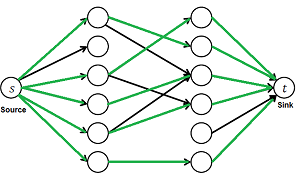
\includegraphics[width=25mm]{content/graph/maximum_matching.png}
\end{center}
\section{Math}
	\subsection{Number of Spanning Trees}
		% I.e. matrix-tree theorem.
		% Source: https://en.wikipedia.org/wiki/Kirchhoff%27s_theorem
		% Test: stress-tests/graph/matrix-tree.cpp
		Crea una $N\times N$ matriz \texttt{mat}, y para cada arista $a \rightarrow b \in G$, hacer
		\texttt{mat[a][b]--, mat[b][b]++} (y \texttt{mat[b][a]--, mat[a][a]++} si $G$ es no dirigido).
		Eliminar la $i$-esima fila y columna y realizar el determinante; esto entrega el numero de arboles de expansion dirigidos con raiz en $i$
		(if $G$ is no dirigifo, eliminar cualquier fila/columna).

	\subsection{Teorema de Erdős–Gallai}
		% Source: https://en.wikipedia.org/wiki/Erd%C5%91s%E2%80%93Gallai_theorem
		% Test: stress-tests/graph/erdos-gallai.cpp
		Un grafo simple con grados $d_1 \ge \dots \ge d_n$ existe si y solo si $d_1 + \dots + d_n$ es par y para cada $k = 1\dots n$,
		\[ \sum _{i=1}^{k}d_{i}\leq k(k-1)+\sum _{i=k+1}^{n}\min(d_{i},k). \]
